\documentclass[10pt]{beamer}
\usetheme[
%%% option passed to the outer theme
%    progressstyle=fixedCircCnt,   % fixedCircCnt, movingCircCnt (moving is deault)
  ]{Feather}
  
% If you want to change the colors of the various elements in the theme, edit and uncomment the following lines

% Change the bar colors:
%\setbeamercolor{Feather}{fg=red!20,bg=red}

% Change the color of the structural elements:
%\setbeamercolor{structure}{fg=red}

% Change the frame title text color:
%\setbeamercolor{frametitle}{fg=blue}

% Change the normal text color background:
%\setbeamercolor{normal text}{fg=black,bg=gray!10}

%-------------------------------------------------------
% INCLUDE PACKAGES
%-------------------------------------------------------

\usepackage[utf8]{inputenc}
\usepackage[english]{babel}
\usepackage[T1]{fontenc}
\usepackage{helvet}
\usepackage{tikz}
\usepackage{graphicx}
\usetikzlibrary{calc,intersections,through,backgrounds,graphs}
\usepackage{pgfcore}
\usepackage{subfig}
\usepackage{float}

%-------------------------------------------------------
% DEFFINING AND REDEFINING COMMANDS
%-------------------------------------------------------

% colored hyperlinks
\newcommand{\chref}[2]{
  \href{#1}{{\usebeamercolor[bg]{Feather}#2}}
}
\def\mathbi#1{\textbf{\em #1}}
%-------------------------------------------------------
% INFORMATION IN THE TITLE PAGE
%-------------------------------------------------------

\title[Digital signal processing on FPGA] % [] is optional - is placed on the bottom of the sidebar on every slide
{ % is placed on the title page
      \textbf{Digital signal processing on FPGA}
}

\subtitle[]
{
      \textbf{}
}

\author[Hossein Beheshti]
{      \textbf{Hossein Beheshti} \\
      {}
}

\institute[]
{
	.\\
  
  %there must be an empty line above this line - otherwise some unwanted space is added between the university and the country (I do not know why;( )
}

\date{\today}

%-------------------------------------------------------
% THE BODY OF THE PRESENTATION
%-------------------------------------------------------
%%%%%%%%%%%%%%%%
%%%%%%%%%%%%%%%%newcommands

\newcommand{\norm}[1]{\left\lVert#1\right\rVert}
%\renewcommand{\rmdefault}{Times New Roman}
%%%%%%%%%
%%%%%%%%%


\usefonttheme[onlymath]{serif} %change font to defult article font


\begin{document}

%-------------------------------------------------------
% THE TITLEPAGE
%-------------------------------------------------------

{\1% % this is the name of the PDF file for the background
\begin{frame}[plain,noframenumbering] % the plain option removes the header from the title page, noframenumbering removes the numbering of this frame only
  \titlepage % call the title page information from above
\end{frame}}

\begin{frame}{Content}{}
\tableofcontents
\end{frame}
%%% change font
\usebeamerfont{body}
%%%%%%%%%%%%% Body
%%%%%%%%%%%%
\section{RFSoC signal transmitter}
%%%%%%%%%%%%%%%%%%%%%%%%%%%%%%%%%%%%%%%%%%%
\begin{frame}{RFSoC signal transceiver}{tx-subsystem}
	\begin{figure}
		\centering
		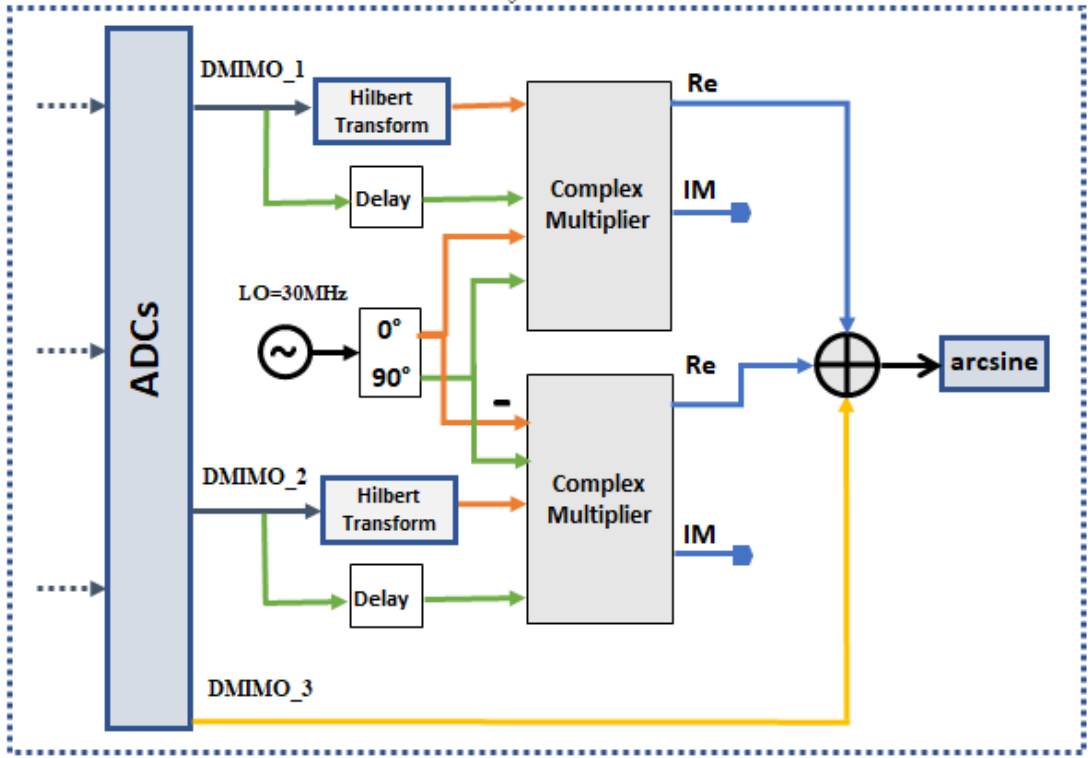
\includegraphics[scale=1]{graphics/tx_ss.png}
		\caption{transmitter subsystem}
	\end{figure}
\end{frame}
%%%%%%%%%%%%%%%%%%%%%%%%%%%%%%%%%%%%%%%%%%%
\begin{frame}{RFSoC signal transceiver}{rx-subsystem}
	\begin{figure}
		\centering
		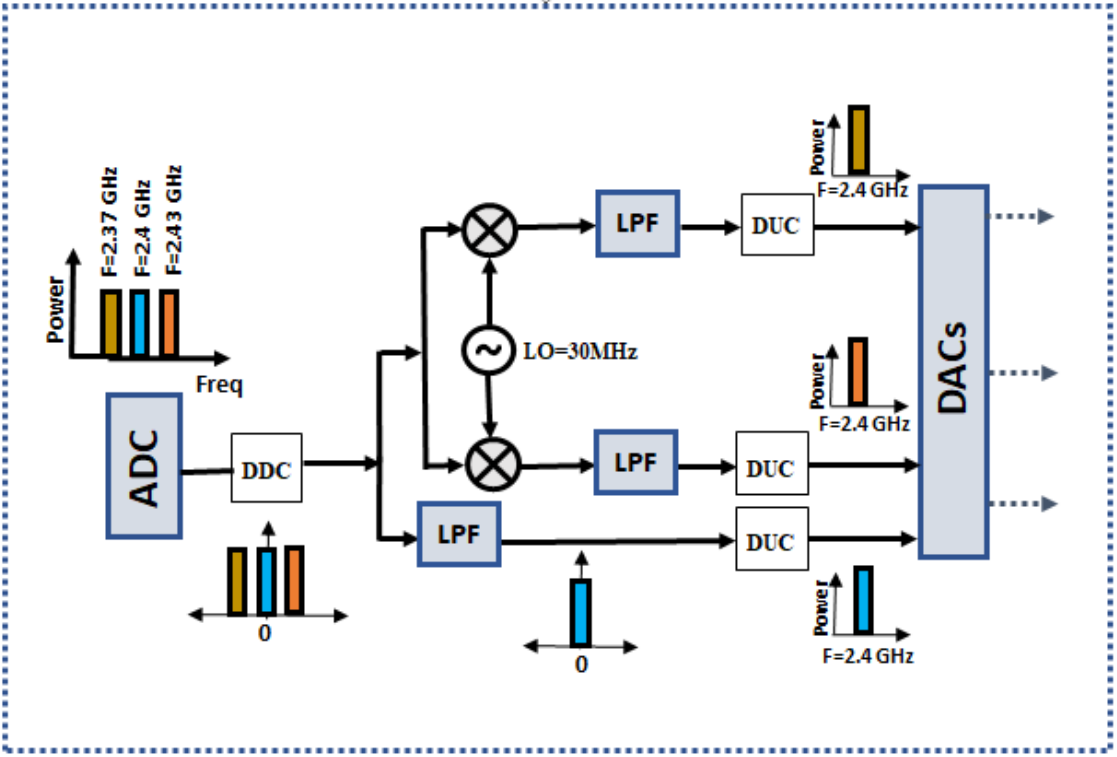
\includegraphics[scale=1]{graphics/rx_ss.png}
		\caption{Receiver subsystem}
	\end{figure}
\end{frame}
%%%%%%%%%%%%
\section{Real-time Spectrum Analyzer}
%%%%%%%%%%%%%%%%%%%%%%%%%%%%%%%%%%%%%%%%%%% 
\begin{frame}{Real-time Spectrum Analyzer}{}
	\begin{block}{Spectrum analyzer type:}
		\begin{itemize}
			\item Swept-tuned spectrum analyzer
			\item Vector signal analyzers
			\item Real-time spectrum analyzers (RTSA)
		\end{itemize}
	\end{block}
	\pause
	\begin{block}{}
		Real-time spectrum analysis allows a spectrum analyzer to conduct continuous,
		gapless capture and analysis of elusive and transient signals, while conventional
		spectrum analyzers and vector signal analyzers do not have this capability due to their design.
	\end{block}
\end{frame}
%%%%%%%%%%%%%%%%%%%%%%%%%%%%%%%%%%%%%%%%%%%
\begin{frame}{Real-time Spectrum Analyzer}{Swept-tuned spectrum analyzer}
	\begin{figure}
		\centering
		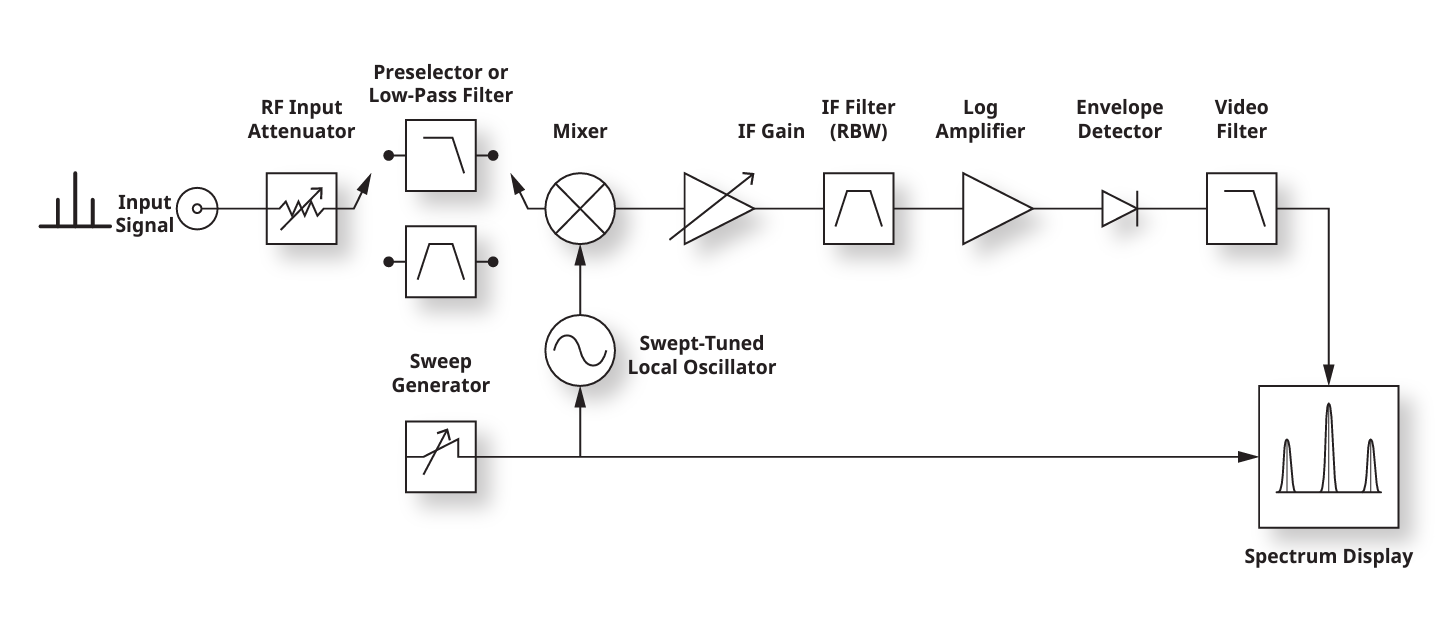
\includegraphics[scale=0.9]{graphics/rtsa_fig1_1.png}
		\caption{Diagram of a classic swept-tuned spectrum analyzer}
	\end{figure}
\end{frame}
%%%%%%%%%%%%%%%%%%%%%%%%%%%%%%%%%%%%%%%%%%%
\begin{frame}{Real-time Spectrum Analyzer}{Swept-tuned spectrum analyzer}
	\begin{figure}
		\centering
		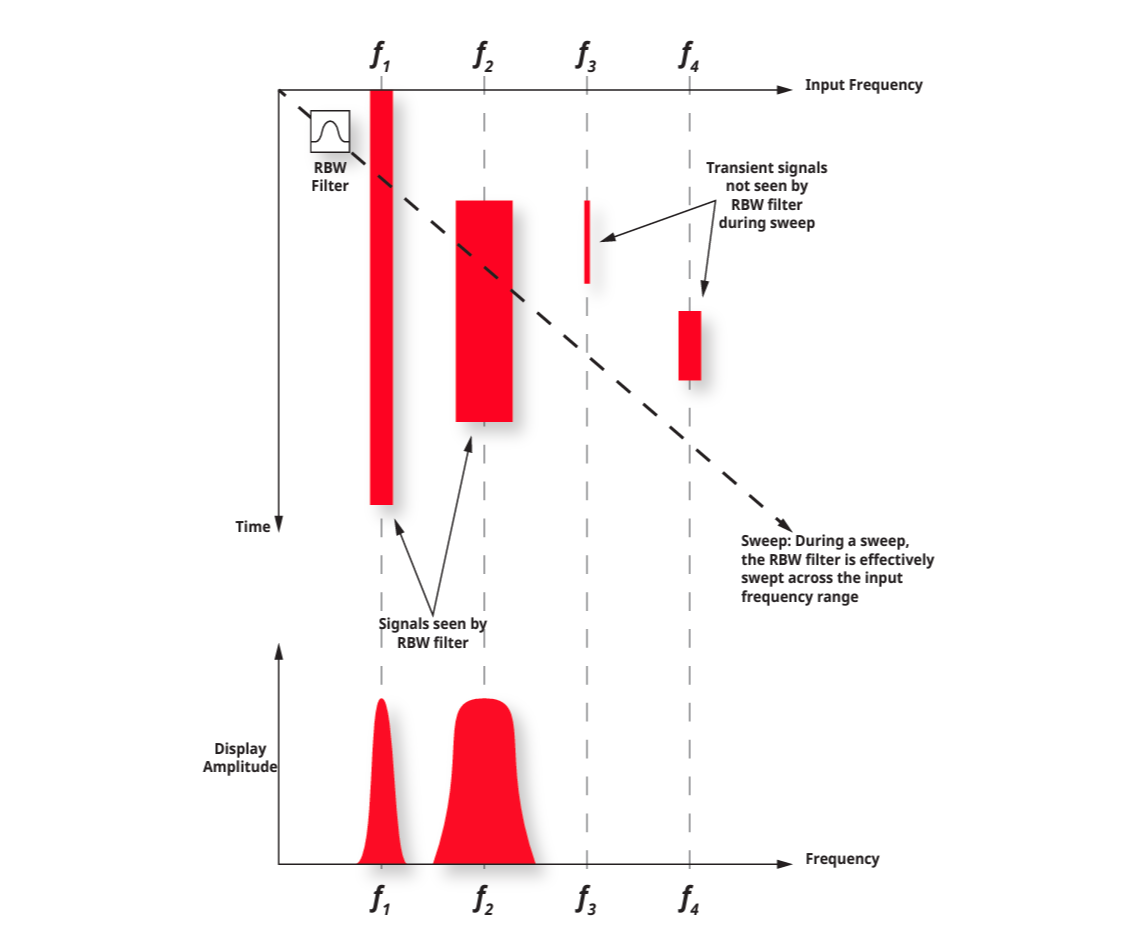
\includegraphics[scale=0.65]{graphics/rtsa_fig1_2.png}
		\caption{Swept-tuned spectrum analyzer response to transient signals during a sweep}
	\end{figure}
\end{frame}
%%%%%%%%%%%%%%%%%%%%%%%%%%%%%%%%%%%%%%%%%%%
\begin{frame}{Real-time Spectrum Analyzer}{Vector signal analyzer}
	\begin{figure}
		\centering
		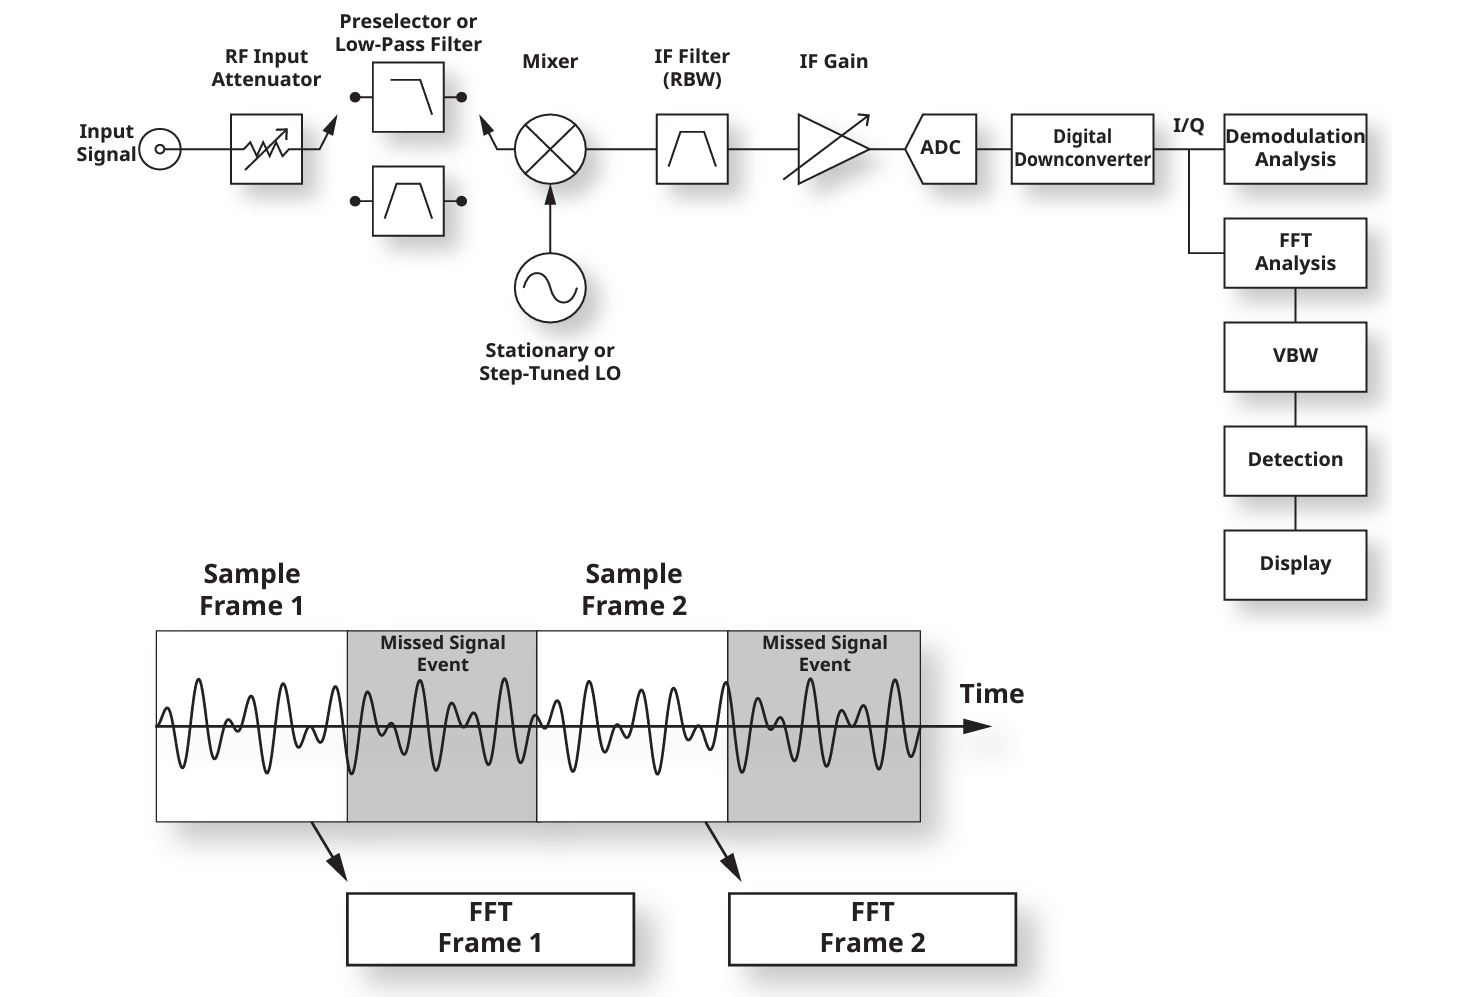
\includegraphics[scale=0.7]{graphics/rtsa_fig2.png}
		\caption{Block diagram of simplified vector signal analyzer and signal processing flow}
	\end{figure}
\end{frame}
%%%%%%%%%%%%%%%%%%%%%%%%%%%%%%%%%%%%%%%%%%%
\begin{frame}{Real-time Spectrum Analyzer}{RTSA}
	\begin{figure}
		\centering
		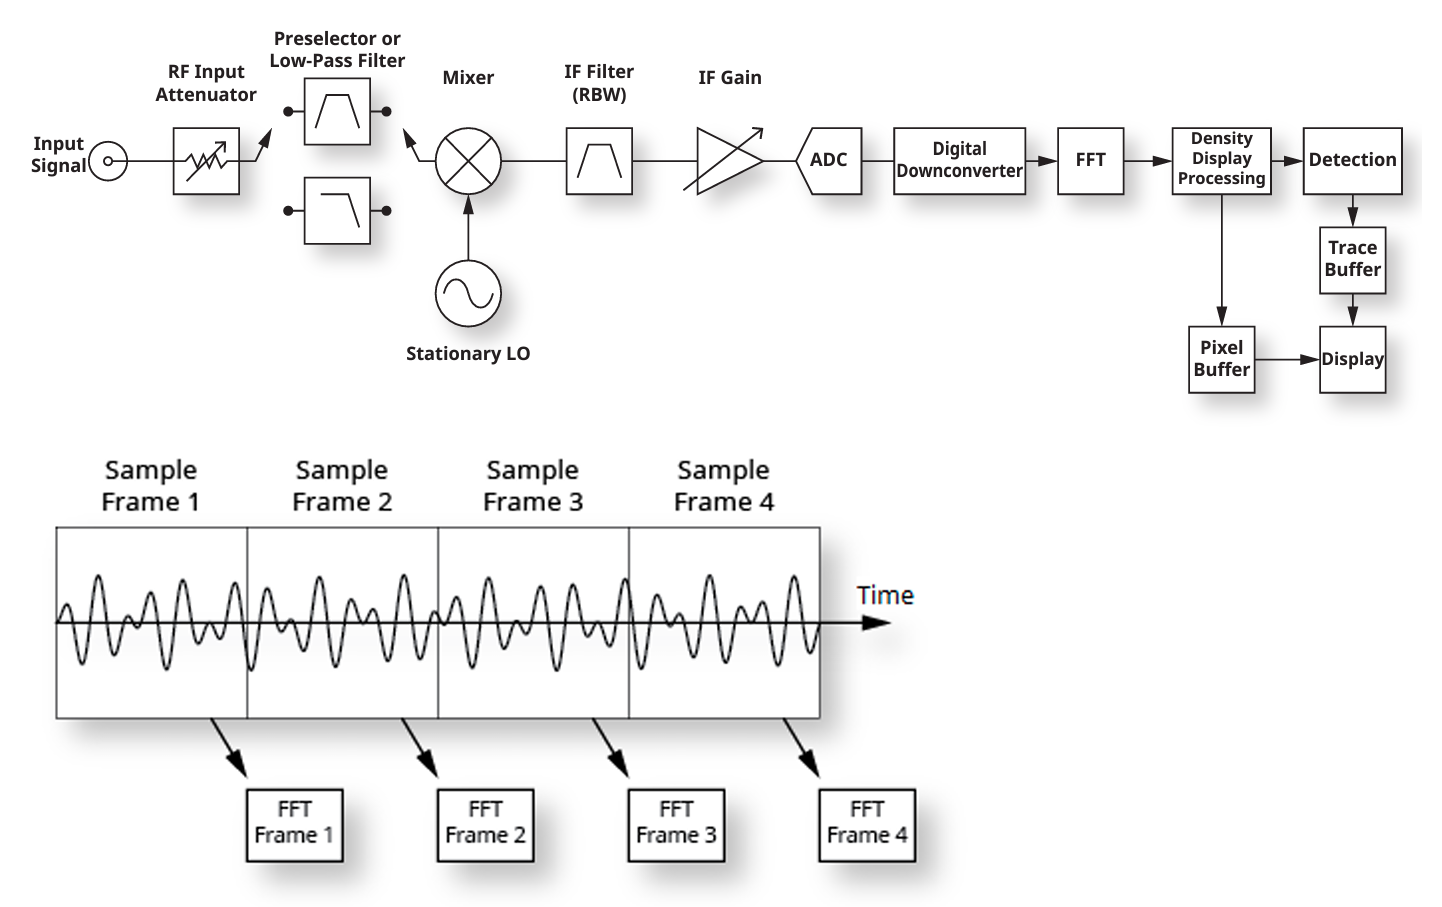
\includegraphics[scale=0.7]{graphics/rtsa_fig3.png}
		\caption{Real-time spectrum analyzer block diagram and signal processing flow}
	\end{figure}
\end{frame}
%%%%%%%%%%%%%%%%%%%%%%%%%%%%%%%%%%%%%%%%%%%
\begin{frame}{Real-time Spectrum Analyzer}{3D-Histogram}
	\begin{figure}
		\centering
		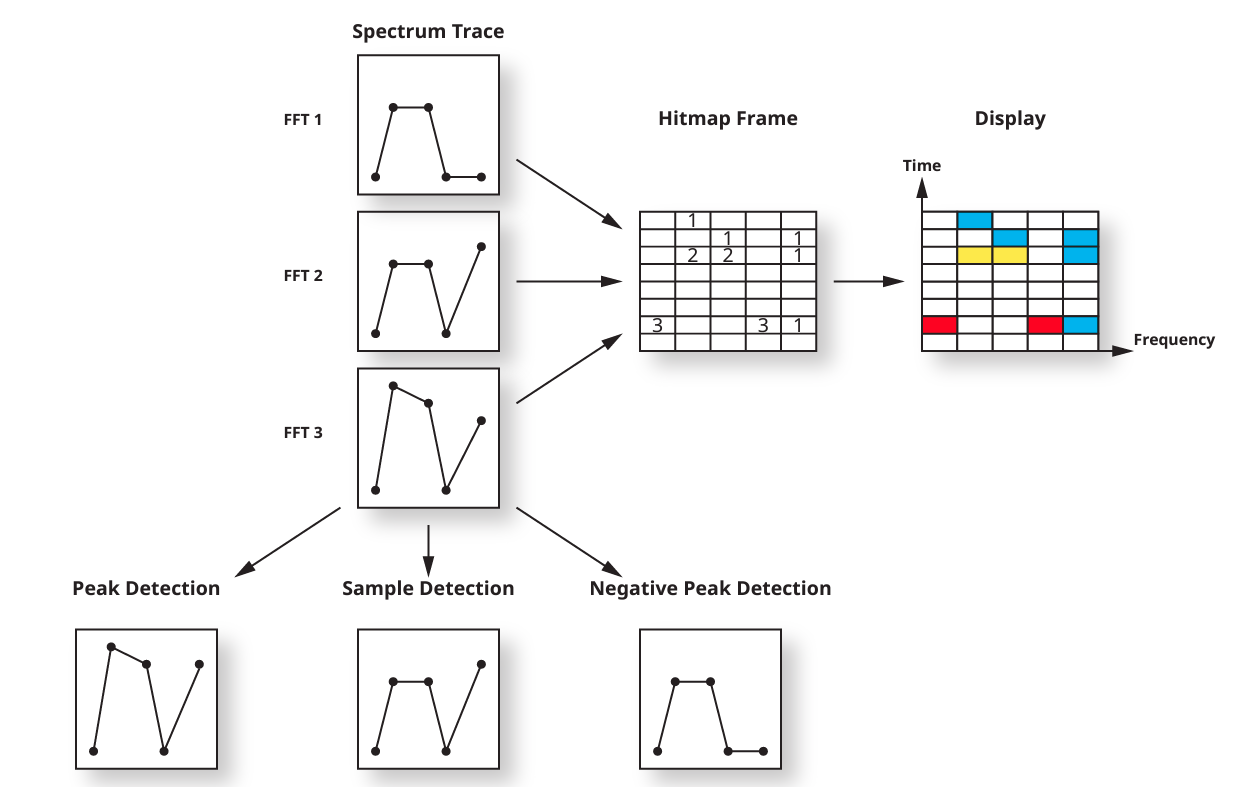
\includegraphics[scale=0.85]{graphics/rtsa_fig4.png}
		\caption{Shows how the spectrum traces are constructed from the detected
			amplitude of all three FFTs acquired during the acquisition time interval}
	\end{figure}
\end{frame}
%%%%%%%%%%%%%%%%%%%%%%%%%%%%%%%%%%%%%%%%%%%
\begin{frame}{Real-time Spectrum Analyzer}{Implementation}
	\begin{figure}
		\centering
		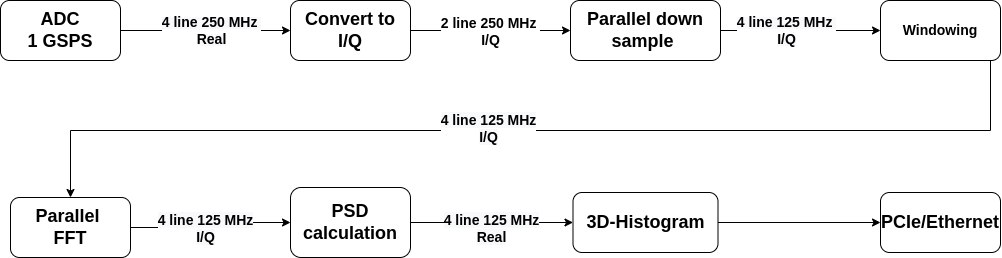
\includegraphics[scale=0.3]{graphics/rtsa_fig5.png}
	\end{figure}
\end{frame}







%%%%%%%%%%%%% The end
{\1
\begin{frame}[plain,noframenumbering]
  \finalpage{\textbf{Thank you}}
\end{frame}}

\end{document}
